\documentclass{standalone}
\usepackage{tikz}
\usetikzlibrary{patterns, positioning}
\usepackage[sfdefault]{ClearSans} %% option 'sfdefault' activates Clear Sans as the default text font
\usepackage[T1]{fontenc}

\begin{document}
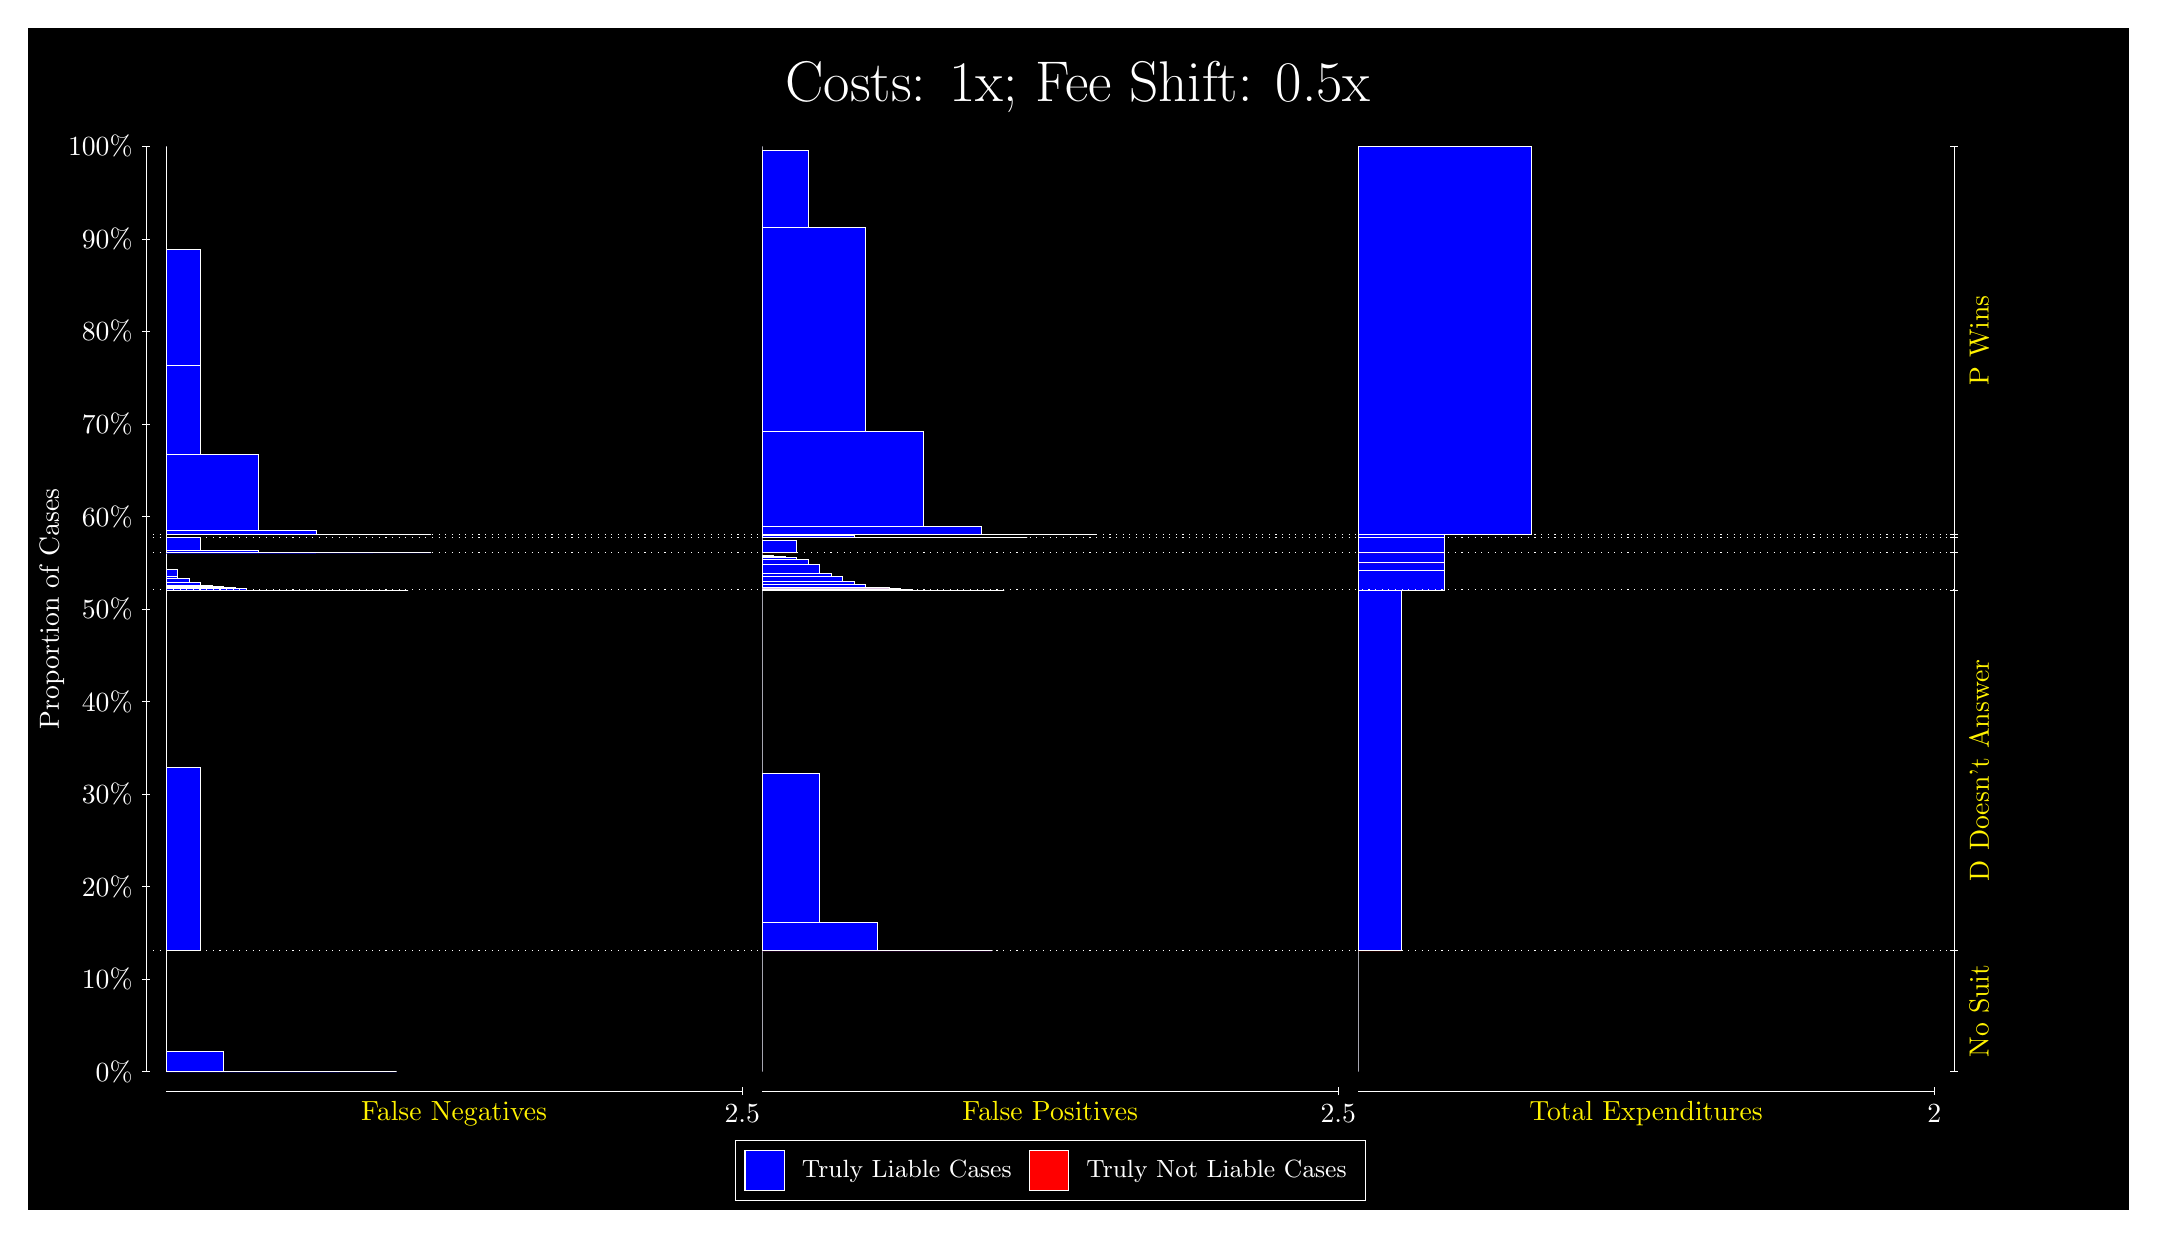
\begin{tikzpicture}
\draw[fill=black] (0,0) rectangle (26.667,15);
\draw[text=white] (0,13.5) rectangle (26.667,15) node[midway] {\huge Costs: 1x; Fee Shift: 0.5x};
\draw[white, very thin] (1.5,1.75) -- (1.5,13.5);
\node[rotate=90, text=white, anchor=center] at (0.3, 7.625) {Proportion of Cases};
\draw[white, very thin] (1.45,1.75) -- (1.55,1.75);
\node[text=white, anchor=east] at (1.45, 1.75) {0\%};
\draw[white, very thin] (1.45,2.925) -- (1.55,2.925);
\node[text=white, anchor=east] at (1.45, 2.925) {10\%};
\draw[white, very thin] (1.45,4.1) -- (1.55,4.1);
\node[text=white, anchor=east] at (1.45, 4.1) {20\%};
\draw[white, very thin] (1.45,5.275) -- (1.55,5.275);
\node[text=white, anchor=east] at (1.45, 5.275) {30\%};
\draw[white, very thin] (1.45,6.45) -- (1.55,6.45);
\node[text=white, anchor=east] at (1.45, 6.45) {40\%};
\draw[white, very thin] (1.45,7.625) -- (1.55,7.625);
\node[text=white, anchor=east] at (1.45, 7.625) {50\%};
\draw[white, very thin] (1.45,8.8) -- (1.55,8.8);
\node[text=white, anchor=east] at (1.45, 8.8) {60\%};
\draw[white, very thin] (1.45,9.975) -- (1.55,9.975);
\node[text=white, anchor=east] at (1.45, 9.975) {70\%};
\draw[white, very thin] (1.45,11.15) -- (1.55,11.15);
\node[text=white, anchor=east] at (1.45, 11.15) {80\%};
\draw[white, very thin] (1.45,12.325) -- (1.55,12.325);
\node[text=white, anchor=east] at (1.45, 12.325) {90\%};
\draw[white, very thin] (1.45,13.5) -- (1.55,13.5);
\node[text=white, anchor=east] at (1.45, 13.5) {100\%};

\draw[white, very thin] (24.457,1.75) -- (24.457,13.5);
\draw[white, very thin] (24.407,1.75) -- (24.507,1.75);
\node[anchor=west] at (24.407, 1.75) {};
\draw[white, very thin] (24.407,3.2846) -- (24.507,3.2846);
\node[anchor=west] at (24.407, 3.2846) {};
\draw[white, very thin] (24.407,7.8662) -- (24.507,7.8662);
\node[anchor=west] at (24.407, 7.8662) {};
\draw[white, very thin] (24.407,8.341) -- (24.507,8.341);
\node[anchor=west] at (24.407, 8.341) {};
\draw[white, very thin] (24.407,8.5324) -- (24.507,8.5324);
\node[anchor=west] at (24.407, 8.5324) {};
\draw[white, very thin] (24.407,8.5712) -- (24.507,8.5712);
\node[anchor=west] at (24.407, 8.5712) {};
\draw[white, very thin] (24.407,13.5) -- (24.507,13.5);
\node[anchor=west] at (24.407, 13.5) {};

\draw[white, very thin, fill=blue] (1.75,1.75) rectangle (4.6775,1.75);
\draw[white, very thin, fill=blue] (1.75,1.75) rectangle (3.9457,1.75);
\draw[white, very thin, fill=blue] (1.75,1.75) rectangle (3.2138,1.7521);
\draw[white, very thin, fill=blue] (1.75,1.7521) rectangle (2.4819,2.0013);
\draw[white, very thin, fill=red] (1.75,2.0013) rectangle (1.75,2.0013);
\draw[white, very thin, fill=blue] (1.75,2.0013) rectangle (1.75,3.2846);
\draw[white, very thin, fill=blue] (1.75,3.2846) rectangle (2.1891,5.6096);
\draw[white, very thin, fill=red] (1.75,5.6096) rectangle (1.75,5.6096);
\draw[white, very thin, fill=blue] (1.75,5.6096) rectangle (1.75,7.8662);
\draw[white, very thin, fill=blue] (1.75,7.8662) rectangle (4.8239,7.8662);
\draw[white, very thin, fill=blue] (1.75,7.8662) rectangle (4.5312,7.8662);
\draw[white, very thin, fill=blue] (1.75,7.8662) rectangle (4.2384,7.8662);
\draw[white, very thin, fill=blue] (1.75,7.8662) rectangle (4.092,7.8662);
\draw[white, very thin, fill=blue] (1.75,7.8662) rectangle (3.9457,7.8662);
\draw[white, very thin, fill=blue] (1.75,7.8662) rectangle (3.7993,7.8662);
\draw[white, very thin, fill=blue] (1.75,7.8662) rectangle (3.6529,7.8662);
\draw[white, very thin, fill=blue] (1.75,7.8662) rectangle (3.5065,7.8662);
\draw[white, very thin, fill=blue] (1.75,7.8662) rectangle (3.3602,7.8663);
\draw[white, very thin, fill=blue] (1.75,7.8663) rectangle (3.2138,7.8663);
\draw[white, very thin, fill=blue] (1.75,7.8663) rectangle (3.0674,7.8664);
\draw[white, very thin, fill=blue] (1.75,7.8664) rectangle (3.0674,7.8664);
\draw[white, very thin, fill=blue] (1.75,7.8664) rectangle (2.921,7.8678);
\draw[white, very thin, fill=blue] (1.75,7.8678) rectangle (2.7746,7.8862);
\draw[white, very thin, fill=blue] (1.75,7.8862) rectangle (2.6283,7.8876);
\draw[white, very thin, fill=blue] (1.75,7.8876) rectangle (2.6283,7.9012);
\draw[white, very thin, fill=blue] (1.75,7.9012) rectangle (2.4819,7.9125);
\draw[white, very thin, fill=blue] (1.75,7.9125) rectangle (2.3355,7.9175);
\draw[white, very thin, fill=blue] (1.75,7.9175) rectangle (2.3355,7.9213);
\draw[white, very thin, fill=blue] (1.75,7.9213) rectangle (2.1891,7.9571);
\draw[white, very thin, fill=blue] (1.75,7.9571) rectangle (2.0428,8.0116);
\draw[white, very thin, fill=blue] (1.75,8.0116) rectangle (2.0428,8.0131);
\draw[white, very thin, fill=blue] (1.75,8.0131) rectangle (1.8964,8.0385);
\draw[white, very thin, fill=blue] (1.75,8.0385) rectangle (1.8964,8.1242);
\draw[white, very thin, fill=blue] (1.75,8.1242) rectangle (1.75,8.1246);
\draw[white, very thin, fill=red] (1.75,8.1246) rectangle (1.75,8.1246);
\draw[white, very thin, fill=blue] (1.75,8.1246) rectangle (1.75,8.341);
\draw[white, very thin, fill=blue] (1.75,8.341) rectangle (5.1167,8.341);
\draw[white, very thin, fill=blue] (1.75,8.341) rectangle (4.3848,8.341);
\draw[white, very thin, fill=blue] (1.75,8.341) rectangle (3.6529,8.3412);
\draw[white, very thin, fill=blue] (1.75,8.3412) rectangle (2.921,8.3704);
\draw[white, very thin, fill=blue] (1.75,8.3704) rectangle (2.1891,8.5324);
\draw[white, very thin, fill=red] (1.75,8.5324) rectangle (1.75,8.5324);
\draw[white, very thin, fill=blue] (1.75,8.5324) rectangle (2.1891,8.5397);
\draw[white, very thin, fill=red] (1.75,8.5397) rectangle (1.75,8.5397);
\draw[white, very thin, fill=blue] (1.75,8.5397) rectangle (1.75,8.5712);
\draw[white, very thin, fill=blue] (1.75,8.5712) rectangle (5.1167,8.5712);
\draw[white, very thin, fill=blue] (1.75,8.5712) rectangle (4.3848,8.5714);
\draw[white, very thin, fill=blue] (1.75,8.5714) rectangle (3.6529,8.6224);
\draw[white, very thin, fill=blue] (1.75,8.6224) rectangle (2.921,9.5944);
\draw[white, very thin, fill=blue] (1.75,9.5944) rectangle (2.1891,10.725);
\draw[white, very thin, fill=blue] (1.75,10.725) rectangle (2.1891,12.19);
\draw[white, very thin, fill=red] (1.75,12.19) rectangle (1.75,12.19);
\draw[white, very thin, fill=blue] (1.75,12.19) rectangle (1.75,13.5);
\draw[white, very thin, fill=red] (9.3189,1.75) rectangle (9.3189,1.75);
\draw[white, very thin, fill=blue] (9.3189,1.75) rectangle (9.3189,3.2846);
\draw[white, very thin, fill=red] (9.3189,3.2846) rectangle (12.246,3.2846);
\draw[white, very thin, fill=blue] (9.3189,3.2846) rectangle (12.246,3.2846);
\draw[white, very thin, fill=blue] (9.3189,3.2846) rectangle (11.515,3.2873);
\draw[white, very thin, fill=blue] (9.3189,3.2873) rectangle (10.783,3.642);
\draw[white, very thin, fill=blue] (9.3189,3.642) rectangle (10.051,5.5412);
\draw[white, very thin, fill=blue] (9.3189,5.5412) rectangle (9.3189,7.8662);
\draw[white, very thin, fill=red] (9.3189,7.8662) rectangle (12.393,7.8662);
\draw[white, very thin, fill=blue] (9.3189,7.8662) rectangle (12.393,7.8662);
\draw[white, very thin, fill=red] (9.3189,7.8662) rectangle (12.1,7.8662);
\draw[white, very thin, fill=blue] (9.3189,7.8662) rectangle (12.1,7.8662);
\draw[white, very thin, fill=red] (9.3189,7.8662) rectangle (11.807,7.8662);
\draw[white, very thin, fill=blue] (9.3189,7.8662) rectangle (11.807,7.8663);
\draw[white, very thin, fill=blue] (9.3189,7.8663) rectangle (11.661,7.8663);
\draw[white, very thin, fill=red] (9.3189,7.8663) rectangle (11.515,7.8663);
\draw[white, very thin, fill=blue] (9.3189,7.8663) rectangle (11.515,7.8663);
\draw[white, very thin, fill=blue] (9.3189,7.8663) rectangle (11.368,7.8663);
\draw[white, very thin, fill=red] (9.3189,7.8663) rectangle (11.222,7.8663);
\draw[white, very thin, fill=blue] (9.3189,7.8663) rectangle (11.222,7.8719);
\draw[white, very thin, fill=blue] (9.3189,7.8719) rectangle (11.075,7.8874);
\draw[white, very thin, fill=red] (9.3189,7.8874) rectangle (10.929,7.8874);
\draw[white, very thin, fill=blue] (9.3189,7.8874) rectangle (10.929,7.8962);
\draw[white, very thin, fill=red] (9.3189,7.8962) rectangle (10.929,7.8962);
\draw[white, very thin, fill=blue] (9.3189,7.8962) rectangle (10.929,7.8962);
\draw[white, very thin, fill=blue] (9.3189,7.8962) rectangle (10.783,7.9028);
\draw[white, very thin, fill=blue] (9.3189,7.9028) rectangle (10.636,7.9037);
\draw[white, very thin, fill=red] (9.3189,7.9037) rectangle (10.636,7.9037);
\draw[white, very thin, fill=blue] (9.3189,7.9037) rectangle (10.636,7.9396);
\draw[white, very thin, fill=blue] (9.3189,7.9396) rectangle (10.49,7.9825);
\draw[white, very thin, fill=red] (9.3189,7.9825) rectangle (10.344,7.9825);
\draw[white, very thin, fill=blue] (9.3189,7.9825) rectangle (10.344,8.035);
\draw[white, very thin, fill=blue] (9.3189,8.035) rectangle (10.197,8.0826);
\draw[white, very thin, fill=blue] (9.3189,8.0826) rectangle (10.197,8.083);
\draw[white, very thin, fill=red] (9.3189,8.083) rectangle (10.051,8.083);
\draw[white, very thin, fill=blue] (9.3189,8.083) rectangle (10.051,8.1941);
\draw[white, very thin, fill=blue] (9.3189,8.1941) rectangle (9.9044,8.1956);
\draw[white, very thin, fill=blue] (9.3189,8.1956) rectangle (9.9044,8.2501);
\draw[white, very thin, fill=blue] (9.3189,8.2501) rectangle (9.758,8.2859);
\draw[white, very thin, fill=blue] (9.3189,8.2859) rectangle (9.6116,8.2948);
\draw[white, very thin, fill=blue] (9.3189,8.2948) rectangle (9.4652,8.306);
\draw[white, very thin, fill=blue] (9.3189,8.306) rectangle (9.4652,8.306);
\draw[white, very thin, fill=blue] (9.3189,8.306) rectangle (9.3189,8.341);
\draw[white, very thin, fill=red] (9.3189,8.341) rectangle (9.758,8.341);
\draw[white, very thin, fill=blue] (9.3189,8.341) rectangle (9.758,8.503);
\draw[white, very thin, fill=blue] (9.3189,8.503) rectangle (9.3189,8.5324);
\draw[white, very thin, fill=red] (9.3189,8.5324) rectangle (12.686,8.5324);
\draw[white, very thin, fill=blue] (9.3189,8.5324) rectangle (12.686,8.5324);
\draw[white, very thin, fill=blue] (9.3189,8.5324) rectangle (11.954,8.5324);
\draw[white, very thin, fill=blue] (9.3189,8.5324) rectangle (11.222,8.5378);
\draw[white, very thin, fill=blue] (9.3189,8.5378) rectangle (10.49,8.5639);
\draw[white, very thin, fill=blue] (9.3189,8.5639) rectangle (9.758,8.5712);
\draw[white, very thin, fill=red] (9.3189,8.5712) rectangle (13.564,8.5712);
\draw[white, very thin, fill=blue] (9.3189,8.5712) rectangle (13.564,8.5712);
\draw[white, very thin, fill=red] (9.3189,8.5712) rectangle (12.832,8.5712);
\draw[white, very thin, fill=blue] (9.3189,8.5712) rectangle (12.832,8.5725);
\draw[white, very thin, fill=red] (9.3189,8.5725) rectangle (12.1,8.5725);
\draw[white, very thin, fill=blue] (9.3189,8.5725) rectangle (12.1,8.6801);
\draw[white, very thin, fill=red] (9.3189,8.6801) rectangle (11.368,8.6801);
\draw[white, very thin, fill=blue] (9.3189,8.6801) rectangle (11.368,9.8811);
\draw[white, very thin, fill=red] (9.3189,9.8811) rectangle (10.636,9.8811);
\draw[white, very thin, fill=blue] (9.3189,9.8811) rectangle (10.636,12.477);
\draw[white, very thin, fill=blue] (9.3189,12.477) rectangle (9.9044,13.449);
\draw[white, very thin, fill=blue] (9.3189,13.449) rectangle (9.3189,13.5);
\draw[white, very thin, fill=red] (16.888,1.75) rectangle (16.888,1.75);
\draw[white, very thin, fill=blue] (16.888,1.75) rectangle (16.888,3.2846);
\draw[white, very thin, fill=red] (16.888,3.2846) rectangle (17.437,3.2846);
\draw[white, very thin, fill=blue] (16.888,3.2846) rectangle (17.437,7.8662);
\draw[white, very thin, fill=red] (16.888,7.8662) rectangle (17.986,7.8662);
\draw[white, very thin, fill=blue] (16.888,7.8662) rectangle (17.986,8.1139);
\draw[white, very thin, fill=red] (16.888,8.1139) rectangle (17.986,8.1139);
\draw[white, very thin, fill=blue] (16.888,8.1139) rectangle (17.986,8.2133);
\draw[white, very thin, fill=red] (16.888,8.2133) rectangle (17.986,8.2133);
\draw[white, very thin, fill=blue] (16.888,8.2133) rectangle (17.986,8.341);
\draw[white, very thin, fill=red] (16.888,8.341) rectangle (17.986,8.341);
\draw[white, very thin, fill=blue] (16.888,8.341) rectangle (17.986,8.5324);
\draw[white, very thin, fill=red] (16.888,8.5324) rectangle (17.986,8.5324);
\draw[white, very thin, fill=blue] (16.888,8.5324) rectangle (17.986,8.5712);
\draw[white, very thin, fill=red] (16.888,8.5712) rectangle (19.083,8.5712);
\draw[white, very thin, fill=blue] (16.888,8.5712) rectangle (19.083,13.5);
\draw[white, dotted] (1.5,3.2846) -- (24.457,3.2846);
\draw[white, dotted] (1.5,7.8662) -- (24.457,7.8662);
\draw[white, dotted] (1.5,8.341) -- (24.457,8.341);
\draw[white, dotted] (1.5,8.5324) -- (24.457,8.5324);
\draw[white, dotted] (1.5,8.5712) -- (24.457,8.5712);
\draw[white, very thin] (1.75,1.5) -- (9.0689,1.5);
\node[text=yellow, anchor=north] at (5.4094, 1.5) {False Negatives};
\draw[white, very thin] (9.0689,1.45) -- (9.0689,1.55);
\node[text=white, anchor=north] at (9.0689, 1.45) {2.5};

\draw[white, very thin] (9.3189,1.5) -- (16.638,1.5);
\node[text=yellow, anchor=north] at (12.978, 1.5) {False Positives};
\draw[white, very thin] (16.638,1.45) -- (16.638,1.55);
\node[text=white, anchor=north] at (16.638, 1.45) {2.5};

\draw[white, very thin] (16.888,1.5) -- (24.207,1.5);
\node[text=yellow, anchor=north] at (20.547, 1.5) {Total Expenditures};
\draw[white, very thin] (24.207,1.45) -- (24.207,1.55);
\node[text=white, anchor=north] at (24.207, 1.45) {2};

\node[text=yellow, centered, rotate=90] at (24.777, 2.5173) {No Suit};
\node[text=yellow, centered, rotate=90] at (24.777, 5.5754) {D Doesn't Answer};



\node[text=yellow, centered, rotate=90] at (24.777, 11.036) {P Wins};

\draw (12.978300999999998,1.5) node[draw=none] (baseCoordinate) {};
\begin{scope}[align=center]
        \matrix[scale=0.5, draw=white, below=0.5cm of baseCoordinate, nodes={draw}, column sep=0.1cm]{
            \node[rectangle, draw, minimum width=0.5cm, minimum height=0.5cm, fill=blue] {}; &
            \node[draw=none, font=\small, text=white] (B) {Truly Liable Cases}; &
            \node[rectangle, draw, minimum width=0.5cm, minimum height=0.5cm, fill=red] {}; &
            \node[draw=none, font=\small, text=white] (B) {Truly Not Liable Cases}; \\
            };
\end{scope}

\end{tikzpicture}
\end{document}